\section{Analisi statica SonarQube}
A causa della mancanza di ulteriori analisi all'interno del plugIn di Checkstyle è stata inserito un ulteriore strumento, ovvero SonaQube \cite{SonarQube}.

Esso è uno strumento che consente ad un team di scrivere codice più pulito e più sicuro. Esso garantisce un'ispezione continua del codice e mette a disposizione migliaia di regole automatizzate finalizzate all’analisi statica del codice. Queste regole forniscono protezione al progetto esaminato e guidano il team di sviluppo.

La home page dello strumento fornisce una fotografia della situazione, in termini di qualità, del progetto sottoposto all’analisi.

Tramite la pagina Issues è possibile valutare in dettaglio ogni problematica trovata, quali sono le issue principali, dove si trovano nel codice e quando sono stati aggiunti.
Per ciascun dominio SonarQube fornisce un diagramma a bolle che mette in correlazione diverse metriche.


\subsection{SonarQube}
\paragraph{Creazione Container SonarQube:}
Per poter utilizzare le funzionalità di sonarqube all'interno del nostro progetto è stato scelto l'implementazione attraverso offerta dal framework Docker, dove viene garantito un ambiente altamente personalizzabile, flessibile e di facile implementazione all'interno di ogni container.
Una volta istanziati i volumi di Docker e modificato il $docker-compose.yaml$, la localhost utilizzata dal componente di sonarqube sarà la porta \textbf{9000}.

\paragraph{Installazione:}
Creati i volumi sono stati inseriti all'interno del $pom.xml$ di maven i seguenti plugin.

\begin{lstlisting}[language=XML, caption={Implementazioni pom.xml}]
    <!-- JaCoCo test coverage -->
    <plugin>
        <groupId>org.jacoco</groupId>
        <artifactId>jacoco-maven-plugin</artifactId>
        <version>0.8.11</version>
        <executions>
            <execution>
                <id>prepare-agent</id>
                <goals>
                    <goal>prepare-agent</goal>
                </goals>
            </execution>
            <execution>
                <id>report</id>
                <goals>
                    <goal>report</goal>
                </goals>
            </execution>
        </executions>
    </plugin>
</plugins>
<pluginManagement>
    <plugins>
        <plugin>
            <!-- SonarQube -->
            <groupId>org.sonarsource.scanner.maven</groupId>
            <artifactId>sonar-maven-plugin</artifactId>
            <version>3.4.0.905</version>
        </plugin>
    </plugins>
</pluginManagement>
</build>
\end{lstlisting}

Come si può notare è stato necessario inserire anche \textbf{Jacoco}\cite{Jacoco} come plugin maven, ovvero una copertura di codice che misura la qualità di un programma che è stato effettivamente eseguito durante un test, così da determinare se il codice è stato testato in modo completo ed efficace.

\paragraph{Come usare SonarQube:}

Una voltà fatto partire il cointainer contenente SonarQube sarà necessario:

\begin{itemize}
 \item accedere all'interfaccia localhost:9000;
 \item inserire user e pasword iniziali (username: admin / password: admin);
 \item modicare la propria password con una propria locale;
 \item creare un nuovo progetto locale impostando nomi e branch desiderati;
 \item generare un \textbf{token} locale e specificare mavem come proprio framework;
 \item lanciare su cmd il proprio comando:
\begin{lstlisting}[style=terminal, 
	caption={Avvio sonarqube}]
    ./mvnw clean verify sonar:sonar -Dsonar.projectKey=GestioneCliente -Dsonar.projectName='GestioneCliente' -Dsonar.host.url=http://localhost:9000 -Dsonar.token=INSERIRE_PROPRIO_TOKEN_SONARQUBE
\end{lstlisting}
\item attendere il fine compilazione e ricaricare la pagina localohost:9000.
\end{itemize}

\subsection{Analisi report SonarQube}
Mostriamo ora significative parti del report generato su alcuni dei nostri microservizi.

\begin{figure}[htbp]
	\centering
	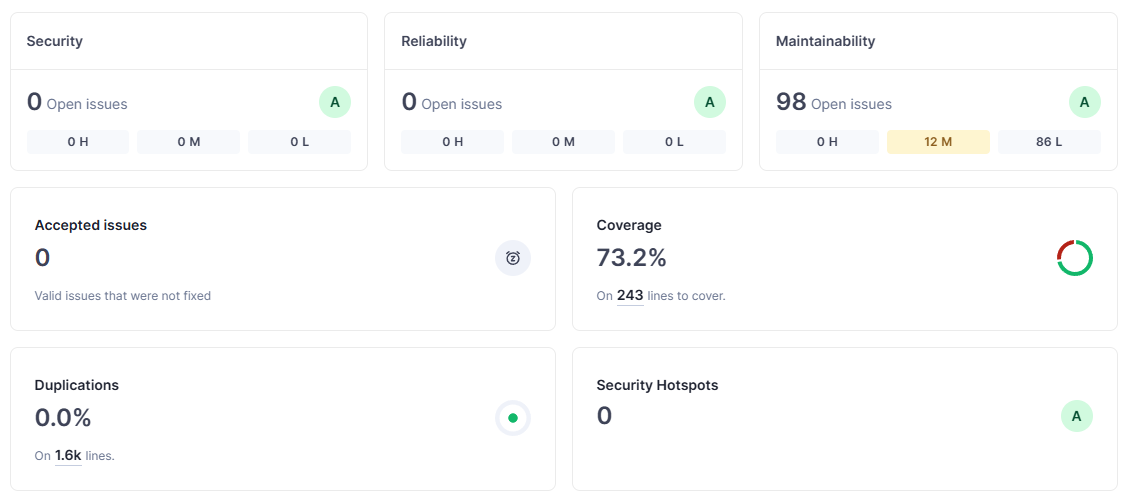
\includegraphics[scale=0.50]{iterazione1/images/Analisys_list_gestione_comanda.png}
	\caption{Analisys list gestione comanda\label{fig:Analisys list gestione comanda}}
\end{figure}

Nella specifica questi controlli servono per:
\begin{itemize}
    \item \textbf{Security (Sicurezza)}:
    \begin{itemize}
        \item La sicurezza del software riguarda la protezione contro le minacce esterne e interne, come hacking, malware e accessi non autorizzati.
        \item Include pratiche come la gestione delle vulnerabilità, l'implementazione di misure di protezione e l'esecuzione di test di sicurezza (penetration testing, security scans).
    \end{itemize}
    \item \textbf{Reliability (Affidabilità)}:
    \begin{itemize}
        \item L'affidabilità del software si riferisce alla capacità del software di funzionare correttamente e senza errori per un periodo di tempo specificato.
        \item Include la gestione degli errori, la ridondanza e la capacità del sistema di recuperare da fallimenti (fault tolerance).
    \end{itemize}
    \item \textbf{Maintainability (Manutenibilità)}:
    \begin{itemize}
        \item La manutenibilità si riferisce alla facilità con cui il software può essere modificato per correggere errori, migliorare le prestazioni o adattarsi a nuovi requisiti.
        \item Comprende aspetti come la leggibilità del codice, la modularità, la documentazione e l'aderenza a standard di codifica.
    \end{itemize}
    \item \textbf{Hotspots Reviewed (Revisioni dei Punti Caldi)}:
    \begin{itemize}
        \item I "punti caldi" sono parti del codice che sono frequentemente modificate o che presentano problemi ricorrenti.
        \item La revisione dei punti caldi implica l'analisi e l'ottimizzazione di queste aree critiche per migliorare la qualità del codice e ridurre il rischio di problemi futuri.
    \end{itemize}
    \item \textbf{Coverage (Copertura)}:
    \begin{itemize}
        \item La copertura del codice si riferisce alla percentuale di codice che viene eseguito durante i test.
        \item Include metriche come la copertura delle linee, delle funzioni e delle condizioni, aiutando a identificare le parti del codice che non sono state testate.
    \end{itemize}
    \item \textbf{Duplications (Duplicazioni)}:
    \begin{itemize}
        \item Le duplicazioni si riferiscono alla presenza di codice duplicato all'interno del progetto software.
        \item Il codice duplicato può aumentare il rischio di errori e rendere il mantenimento più difficile. Rimuovere le duplicazioni aiuta a mantenere il codice più pulito e manutenibile.
    \end{itemize}
\end{itemize}

\newpage
Alcune immagini create per mostrare i test di sonarqube che permettono di individuare le parti di maggior interesse.
Esse Vengono rappresentate anche attraverso grafici di bole facilmente leggibili e interattivi.

\begin{figure}[htbp]
	\centering
	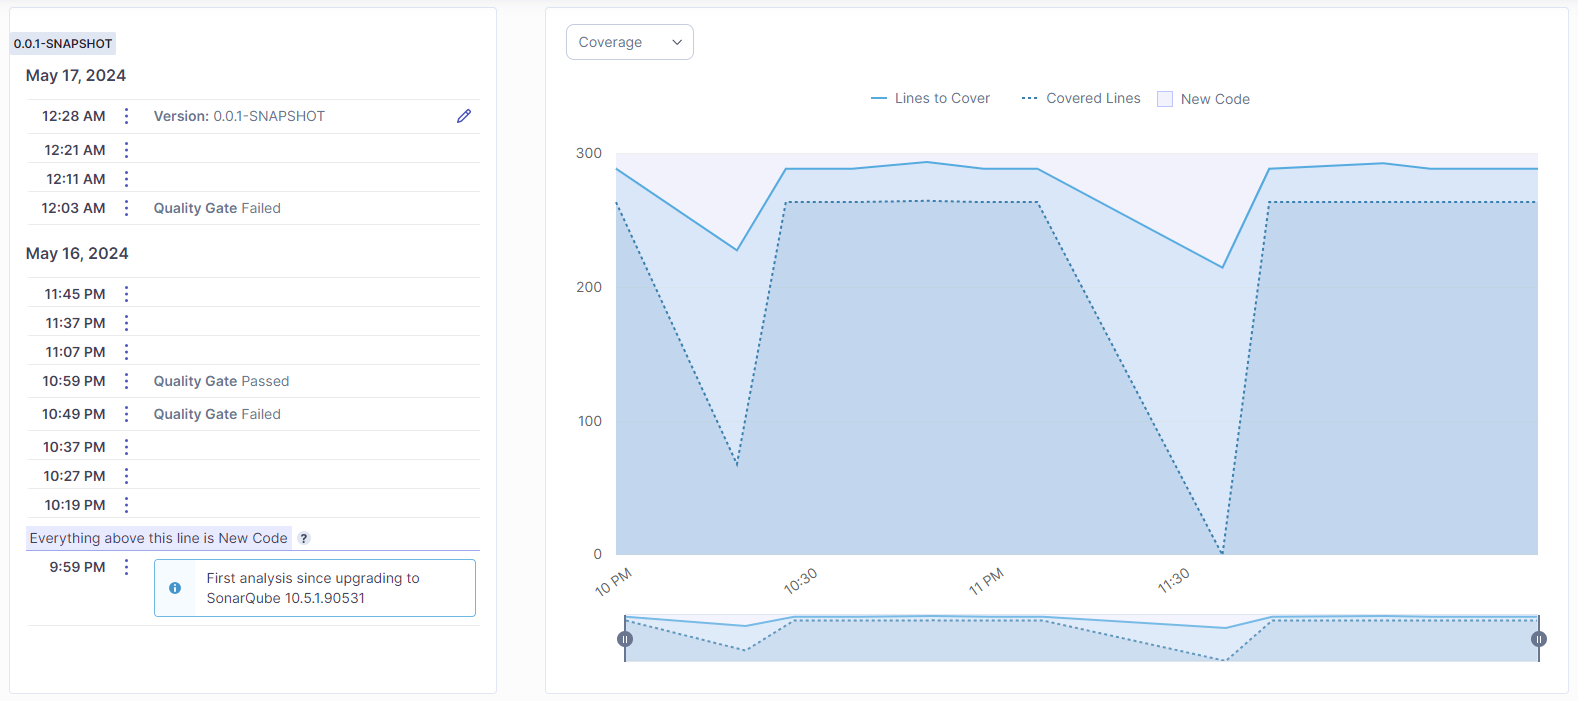
\includegraphics[scale=0.30]{iterazione1/images/coverage_percent_modifier.png}
	\caption{Coverage variata nel corso delle modifiche testate\label{fig:coverage percent modifier}}
\end{figure}

\begin{figure}[htbp]
	\centering
	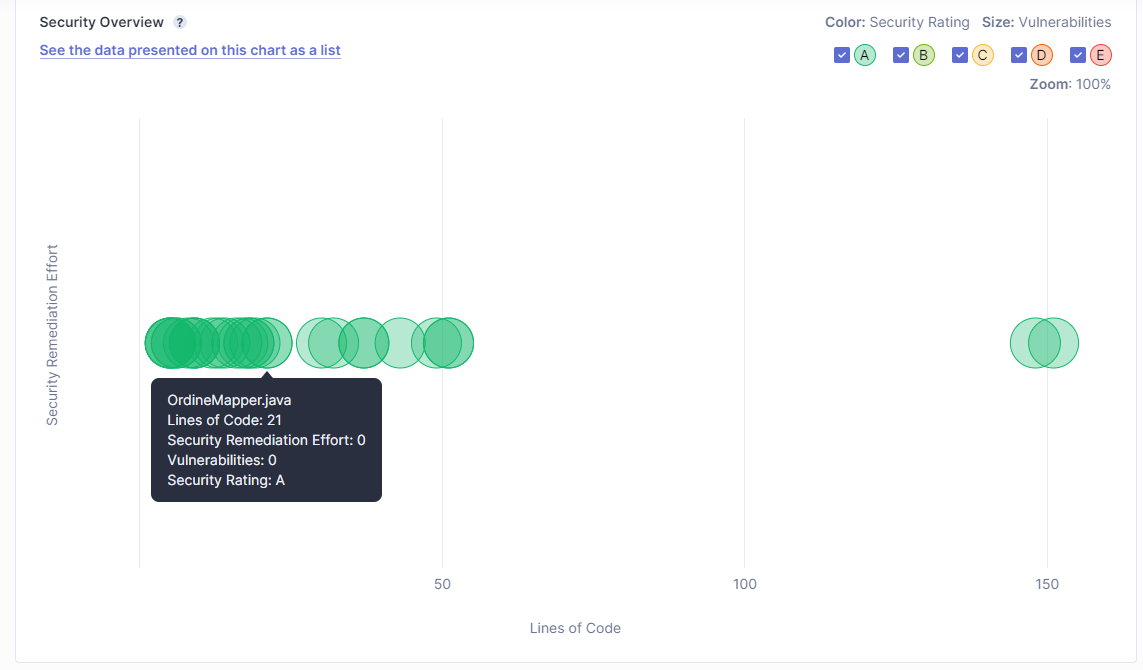
\includegraphics[scale=0.50]{iterazione1/images/secutiry.png}
	\caption{diagramma di bole sulla secutity\label{fig:security}}
\end{figure}

\begin{figure}[htbp]
	\centering
	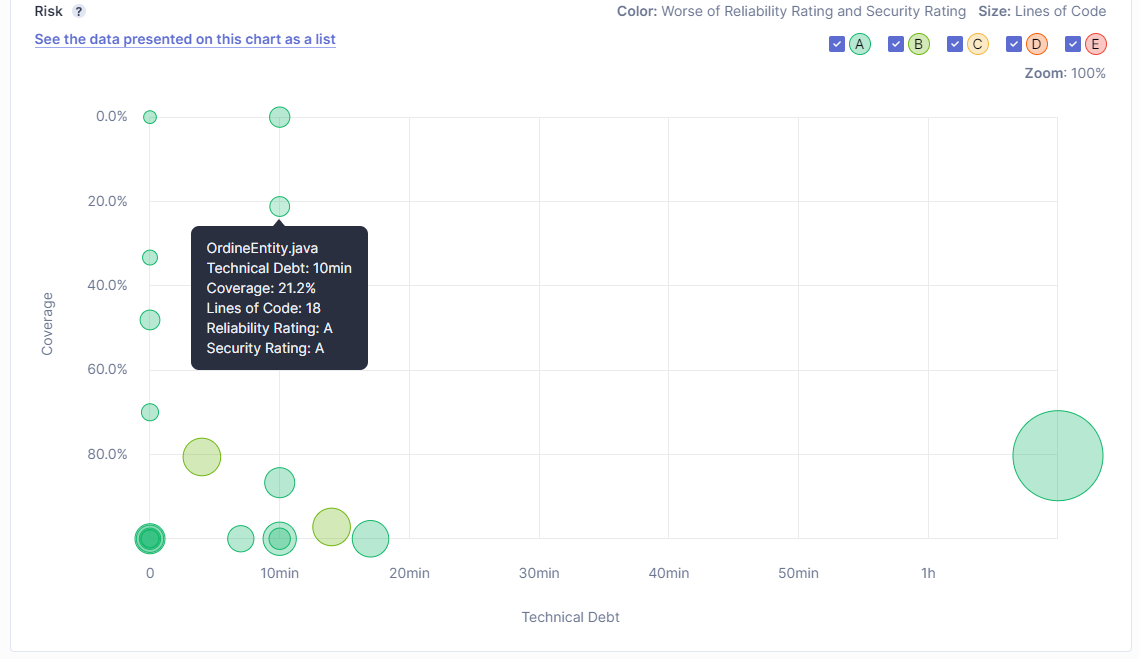
\includegraphics[scale=0.50]{iterazione1/images/risk.png}
	\caption{diagramma di bole sui risk\label{fig:risk}}
\end{figure}

\begin{figure}[htbp]
	\centering
	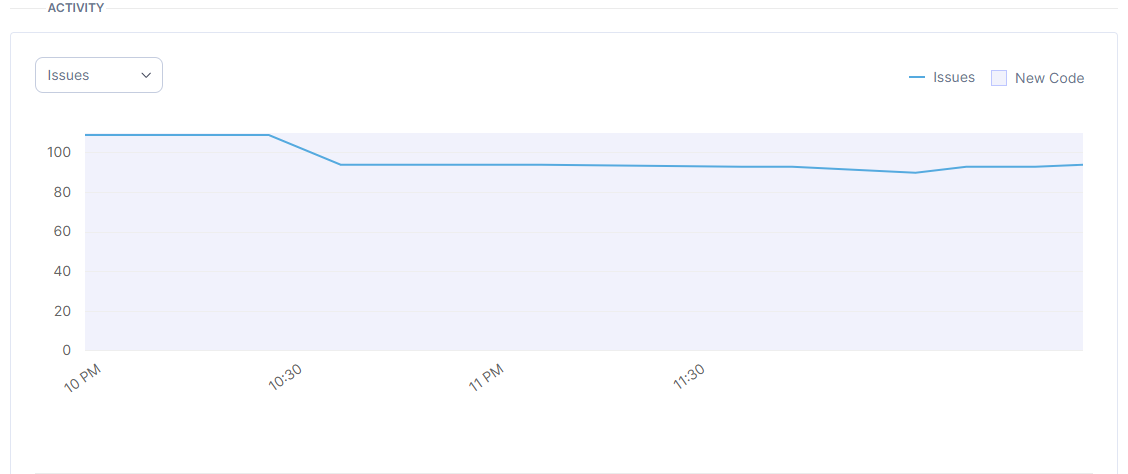
\includegraphics[scale=0.50]{iterazione1/images/issues.png}
	\caption{overview issues\label{fig:issues}}
\end{figure}

\begin{figure}[htbp]
	\centering
	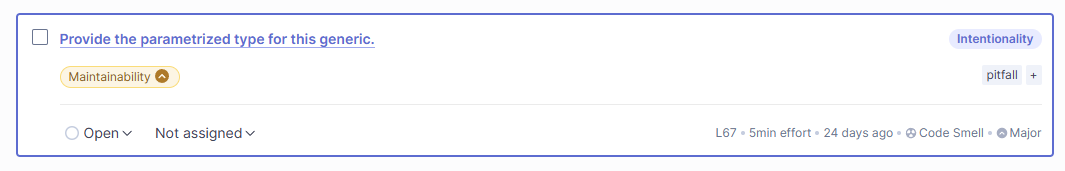
\includegraphics[scale=0.50]{iterazione1/images/visione_issue.png}
	\caption{issues specifico\label{fig:visione issues}}
\end{figure}

\begin{figure}[htbp]
	\centering
	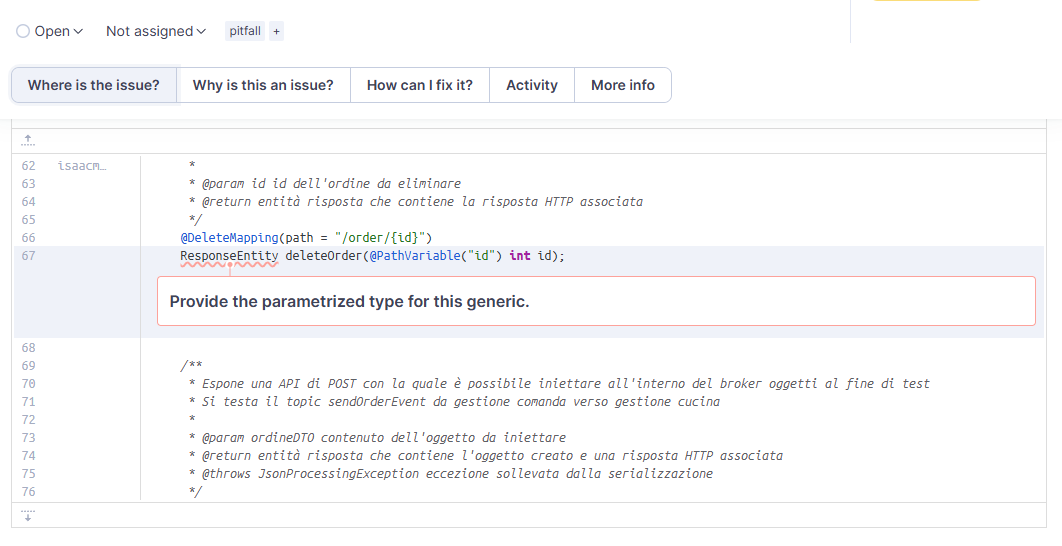
\includegraphics[scale=0.50]{iterazione1/images/esempio_issue.png}
	\caption{view singolo issue\label{fig:esempio issue}}
\end{figure}

\begin{figure}[htbp]
	\centering
	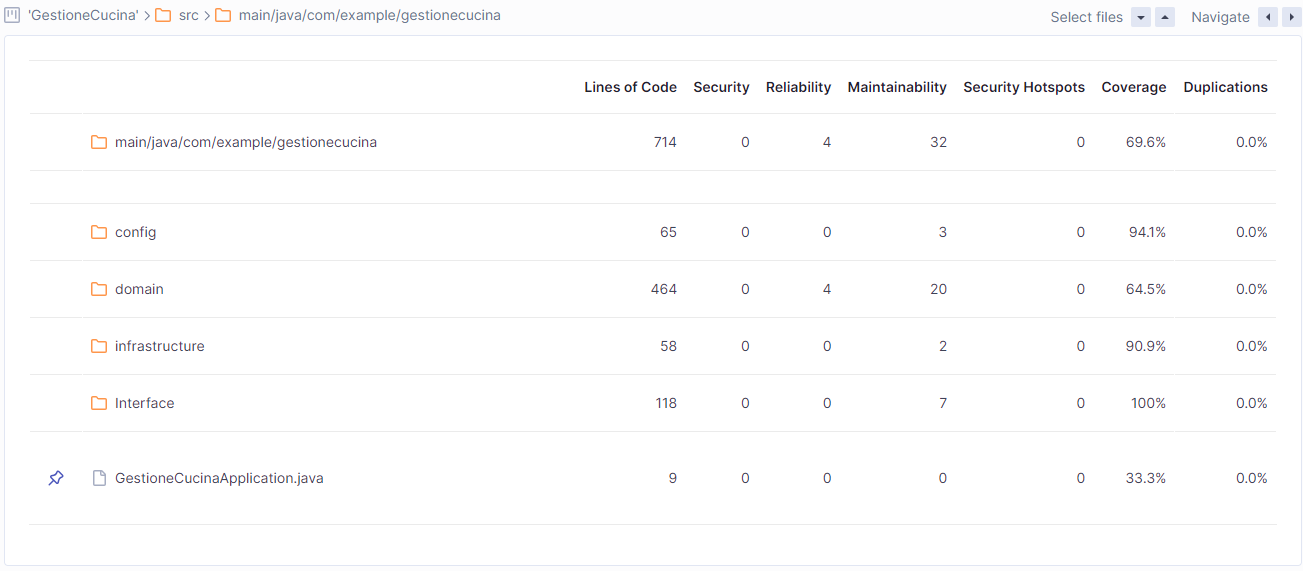
\includegraphics[scale=0.40]{iterazione1/images/gestione_cucina_overview.png}
	\caption{gestione cucina overview\label{fig:gestione cucina overview}}
\end{figure}

\begin{figure}[htbp]
	\centering
	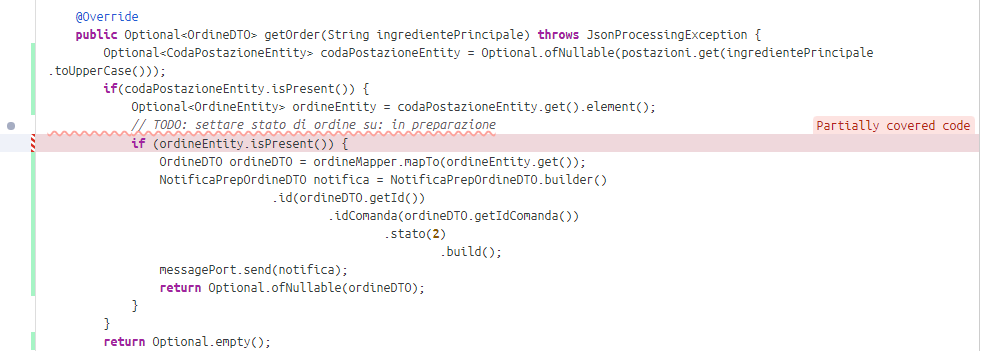
\includegraphics[scale=0.60]{iterazione1/images/esempio_caso_uncoverage.png}
	\caption{esempio caso uncoverage\label{fig:esempio caso uncoverage}}
\end{figure}

Una breve Panoramica delle rules di java esistenti su SonarQube, ognuna di esse può essere totalmente modificata.
\begin{figure}[htbp]
	\centering
	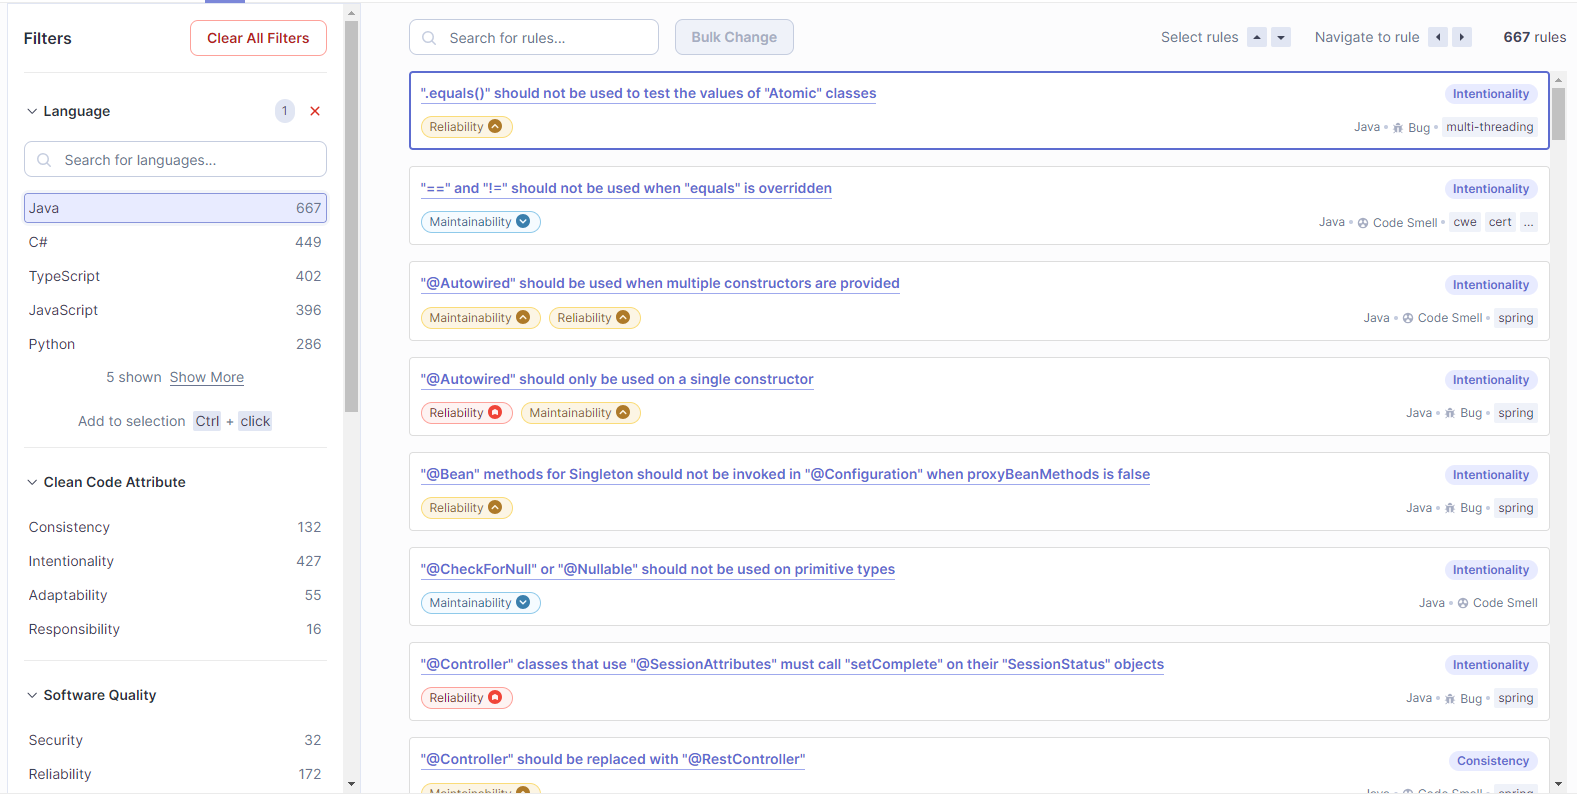
\includegraphics[scale=0.30]{iterazione1/images/java_rules.png}
	\caption{java rules overview sonarqube\label{fig:java rules}}
\end{figure}

\clearpage